\chapauthor{Ковалёв М.В.\\Крощенко А.А.\\Головко В.А.}
\chapter{Конвергенция и интеграция искусственных нейронных сетей с базами знаний в интеллектуальных компьютерных системах нового поколения}
\chapauthortoc{Ковалёв М.В.\\Крощенко А.А.\\Головко В.А.}
\label{chapter_ann}

\abstract{В последнее десятилетие все больше назревает необходимость в разработке гибридных интеллектуальных систем. В контексте этого особое значение приобретают системы, разработанные с использованием семантической технологии (например, \scnkeyword{Технологии OSTIS}) и искусственных нейронных сетей (\scnkeyword{и.н.с.}). Такие гибридные системы обладают достоинствами, которые недостижимы при использовании отдельных технологий. С одной стороны, здесь используются нейронные сети, которые могут работать с неструктурированными и плохо формализованными данными. С другой стороны, применяются семантические технологии, благодаря которым можно объяснить работу любого ``черного'' ящика. Все это формирует серьезную основу для разработки систем, способных не только к эффективной обработке данных, но и к интерпретации получаемых на каждом этапе результатов.} 

\section{Модели искусственных нейронных сетей, используемых в ostis-системах}

Преимущество \scnkeyword{и.н.с.} заключается в том, что они могут работать с неструктурированными данными.
Главный недостаток \scnkeyword{и.н.с.} -- это отсутствие понятной человеку обратной связи, которую можно было бы назвать цепочкой
рассуждений, т.е. можно сказать, что \scnkeyword{и.н.с.} работают по принципу ``черного ящика'' [\scncite{gastelvecchi2016}].

Сложность современных интеллектуальных систем, использующих нейросетевые модели, а также большой объём обрабатываемых ими данных обуславливают необходимость объяснения и мониторинга механизмов их работы с целью оценки их деятельности и ее оптимизации.

В связи с этим актуальность приобретает разработка нейросимволических подходов (описанных, например, в работе [\scncite{nesy1}], в частности, подходов по интеграции \scnkeyword{и.н.с.} и баз знаний, использующих онтологии. Такие интегрированные системы способны сочетать работу \scnkeyword{и.н.с.} по извлечению скрытых закономерностей из массива данных с возможностью их семантической интерпретации чисто символическими подходами ИИ. Это позволяет более точно описать свойства \scnkeyword{и.н.с.}, ее состояния, что в свою очередь делает возможным приоткрыть завесу неопределенности над процессами, скрытыми в ``черном ящике'' [\scncite{ann_ostis2018}].

Можно выделить два основных направления интеграции \scnkeyword{и.н.с.} с базами знаний:

\begin{itemize}
	\item построение интеллектуальных систем, использующих нейросетевые методы наравне с другими имеющимися в системе методами для решения задач или подзадач системы. Такие системы смогут учитывать семантику решаемых задач на более высоком уровне, что сделает решение этих задач структурированными и понятным.

	\item построение интеллектуальной среды по разработке, обучению и интеграции различных \scnkeyword{и.н.с.}, совместимых с базами знаний через представление структур \scnkeyword{и.н.с.} с помощью онтологического подхода и их интерпретацию средствами представления знаний.
	
	\item исследование влияния входных данных на выход нейронных сетей с формулированием правил, которые могут быть погружены в БЗ.
\end{itemize}

Такая среда предоставит возможности интроспекции \scnkeyword{и.н.с.}, сохранения состояний \scnkeyword{и.н.с.} после обучения и реконфигурации сети с целью улучшения ее качеств.

Таким образом, станет возможным проводить более глубокий анализ работы \scnkeyword{и.н.с.}. С другой стороны, формальное описание знаний в рамках предметной области \scnkeyword{и.н.с.} уменьшит порог вхождения разработчиков в теорию методов решения задач с помощью \scnkeyword{и.н.с.}

Данный раздел посвящен предметной области и онтологии искусственных нейронных сетей, используемых в ostis-системах

\subsection{Синтаксис моделей искусственных нейронных сетей, используемых в ostis-системах}

Используя \textit{SC-код}, искусственную нейронную сеть можно определить как 

\begin{SCn}
	\scnheader{искусственная нейронная сеть}
	\scnidtf{и.н.с.}
	\scnidtf{множество искусственных нейронных сетей}
	\scnidtf{нейронная сеть}
	\scntext{пояснение}{Cовокупность нейронных элементов и связей между ними [\scncite{Golovko2017}].}
\end{SCn}

Искусственная нейронная сеть состоит из \scnkeyword{формальных нейронов}, которые связаны между собой посредством \scnkeyword{синаптических связей}. Нейроны организованы в \scnkeyword{слои}. Каждый нейрон слоя принимает сигналы с входящих в него синаптических связей, обрабатывает их единым образом с помощью заданной ему или всему слою \scnkeyword{функции активации} и передает результат на следующий слой нейронных элементов. Структура и характеристики слоев определяют порядок обработки информации в нейронной сети.

Пример архитектуры и.н.с. представлен на рисунке \textit{\nameref{fig:nn_example}}.

\begin{figure}[H]
	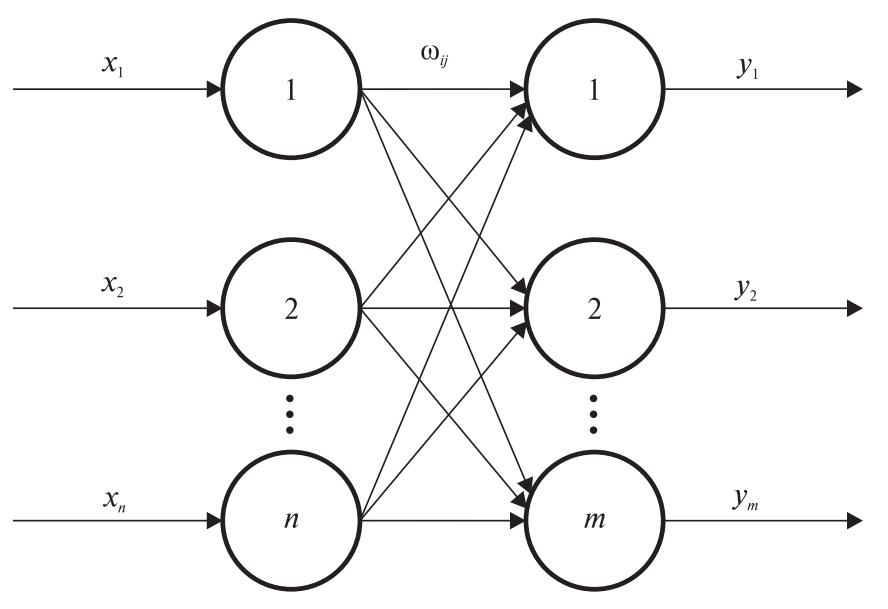
\includegraphics[scale=0.3]{author/part3/figures/neural_network.png}
	\caption{Пример архитектуры и.н.с.}
	\label{fig:nn_example}
\end{figure}

	Такая формулировка предполагает существование определенной нейросетевой архитектуры, которая определяет структурную конфигурацию модели.
	
	Рассмотрим архитектурные компоненты подробнее.

\begin{SCn}
	\scnheader{формальный нейрон}
	\scnidtf{искусственный нейрон}
	\scnidtf{нейрон}
	\scnidtf{ф.н.}
	\scnidtf{нейронный элемент}
	\scnidtf{множество нейронов искусственных нейронных сетей}
	\scnidtf{математическая модель биологического нейрона}
	\scnsubset{искусственная нейронная сеть}
	\scntext{пояснение}{Основной элемент \scnkeyword{и.н.с.}, применяющий свою \scnkeyword{функцию активации} [\scncite{Golovko2017}] к сумме произведений входных сигналов на весовые коэффициенты:
	\begin{equation*}
		y = F\left(\sum_{i=1}^{n} w_ix_i - T\right) = F(WX - T)
	\end{equation*}
	где $X = (x_1,x_2,...,x_n)^{T}$ -- вектор входного сигнала; $W - (w_1,w_2,...,w_n)$ -- вектор весовых коэффициентов; \textit{T} -- пороговое значение;
	\textit{F} -- \scnkeyword{функция активации}.}
\end{SCn}

Отдельный формальный нейрон является искусственной нейронной сетью с одним нейроном в единственном слое.

Пример описания одного нейрона в SCg представлен на рисунке \textit{\nameref{fig:nn_scg}}.

\begin{figure}[H]
	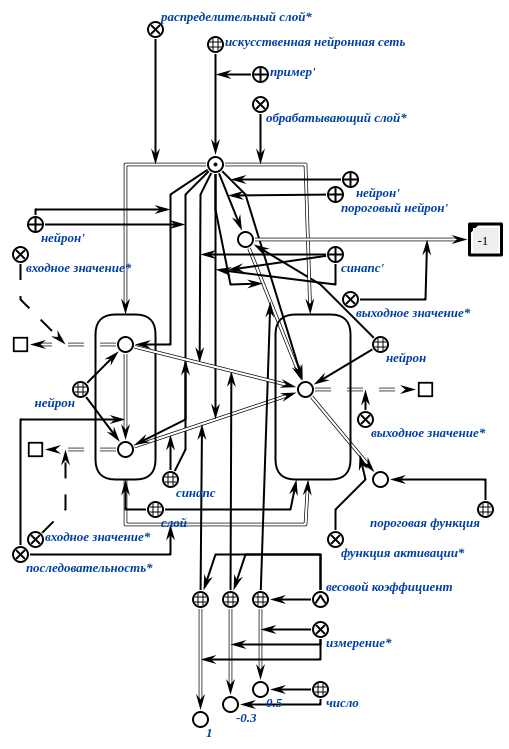
\includegraphics[scale=0.8]{author/part3/figures/neural_network_scg.png}
	\caption{Представление одного нейрона в SCg}
	\label{fig:nn_scg}
\end{figure}

Формальные нейроны могут быть классифицированы следующим образом:

\begin{itemize}
		\item полносвязный формальный нейрон -- нейрон, у которого есть полный набор связей с нейронами предшествующего слоя. Oтдельный обрабатывающий элемент \scnkeyword{и.н.с.}, выполняющий функциональное преобразование взвешенной суммы элементов вектора входных значений с помощью \scnkeyword{функции активации}
	 \item сверточный формальный нейрон -- отдельный обрабатывающий элемент \scnkeyword{и.н.с.}, выполняющий функциональное преобразование результата операции свертки матрицы входных значений с помощью \scnkeyword{функции активации}. Сверточный \scnkeyword{формальный нейрон} может быть представлен полносвязным \scnkeyword{формальным нейроном}.
	\item рекуррентный \scnkeyword{формальный нейрон} -- нейрон, имеющий обратную связь с самим собой или с другими нейронами \scnkeyword{и.н.с.}
\end{itemize}

Схематически формальный нейрон можно представить в виде следующей модели (рисунок \textit{\nameref{fig:formal_neuron}}).

\begin{figure}[H]
	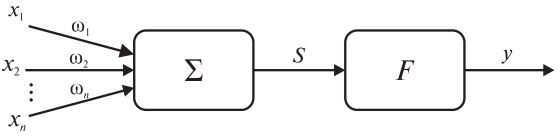
\includegraphics[scale=0.8]{author/part3/figures/formal_neuron.png}
	\caption{Формальный нейрон}
	\label{fig:formal_neuron}
\end{figure}

Определим понятие \scnkeyword{синаптическая связь} и \scnkeyword{слой и.н.с.}:

\begin{SCn}
	\scnheader{синаптическая связь}
	\scnidtf{синапс}
	\scnsubset{ориентированная пара}
	\scntext{пояснение}{ориентированная пара, первым компонентом которой является нейрон, из
	которого исходит сигнал, а вторым компонентом -- нейрон, который принимает этот сигнал}
\end{SCn}


\begin{SCn}
	\scnheader{слой и.н.с.}
	\scnidtf{слой}
	\scnidtf{слой искусственной нейронной сети}
	\scnidtf{множество слоев искусственных нейронных сетей}
	\scnsubset{искусственная нейронная сеть}
	\scntext{пояснение}{множество нейронных элементов, на которые в каждый такт времени
		параллельно поступает информация от других нейронных элементов сети [\scncite{Golovko2017}]}
	\scntext{пояснение}{множество формальных нейронов, осуществляющих параллельную независимую обработку вектора или матрицы входных значений}
\end{SCn}

Отдельный слой является искусственной нейронной сетью с одним слоем.

Следует отметить принципиальную важность этого замечания. Один \scnkeyword{слой и.н.с.}  уже является нейронной сетью, поскольку над ним можно производить все основные операции, которые производятся над ``большой'' \scnkeyword{и.н.с.} (его можно обучить и использовать для решения определенной задачи).

\scnkeyword{Слои и.н.с.} могут быть классифицированы следующим образом (по признаку операции, осуществляемой слоем):
\begin{itemize}
		\item полносвязный слой и.н.с. -- слой, в котором каждый нейрон является полносвязным
		\item сверточный слой и.н.с. -- слой, в котором каждый нейрон является сверточным
		\item слой и.н.с. нелинейного преобразования -- слой, осуществляющий нелинейное преобразование входных данных
		\item dropout слой и.н.с. -- слой, реализующий технику регуляризации dropout
		\item pooling слой и.н.с. -- подвыборочный слой
		\item слой и.н.с. батч-нормализации
\end{itemize}

Как правило, слой нелинейного преобразования  выделяется в отдельный слой только в программных реализациях. Фактически он рассматривается как финальный этап расчета выходной активности любого нейрона -- применение \scnkeyword{функции активации}.

Dropout-слой функционирует только во время обучения \scnkeyword{и.н.с.} Поскольку полносвязные слои имеют большое количество настраиваемых параметров, они подвержены эффекту \scnkeyword{переобучения}. Один из способов устранить такой негативный эффект -- выполнить частичный отсев результатов на выходе полносвязного слоя. На этапе обучения техника dropout позволяет отбросить выходную активность некоторых нейронов с определенной, заданной вероятностью. Выходная активность ``отброшенных'' нейронов полагается равной нулю.

Назначение подвыборочного слоя -- в осуществлении уменьшения размерности входных данных.

Нужно отметить, что данный перечень неполный -- разновидности \scnkeyword{слоев и.н.с.} появляются практически в каждой заслуживающей внимания публикации по нейросетевым алгоритмам и на текущий момент их существует достаточно много, однако, как правило, при построении более традиционных архитектур ограничиваются только приведенными вариантами слоев.

\scnkeyword{Слои и.н.с.} также могут быть классифицированы по исполняемой роли в рамках архитектуры (место в последовательности \scnkeyword{слоев и.н.с.}).

Так, например, слой, расположенный первым, называется распределяющим. Слои, расположенные далее, за исключением последнего, называются обрабатывающими. Наконец, последний слой носит название выходного \scnkeyword{слоя и.н.с.}

Наконец, последний архитектурный компонент \scnkeyword{и.н.с.} -- это функция активации:

\begin{SCn}
	\scnheader{функция активации*}
	\scnidtf{функция активации нейрона*}
	\scniselement{неролевое отношение}
	\scniselement{бинарное отношение}
	\scntext{пояснение}{неролевое отношение, связывающее формальный нейрон с функцией, результат
		применения которой к \textbf{\textit{взвешенной сумме нейрона}} определяет его \textbf{\textit{выходное значение}}.}
	%\scnrelfrom{область определения}{
		
	%}
    %\scnreltoset{объединение}{формальный нейрон;функция}
	\scnrelfrom{первый домен}{формальный нейрон}
	\scnrelfrom{второй домен}{функция}
\end{SCn}

Перечислим некоторые, наиболее известные и применяемые типы функций активации:
\begin{itemize}
	\item линейная функция\\
	\scntext{формула}{
		\begin{equation*}
			y = kS
		\end{equation*}
		где \textit{k} -- коэффициент наклона прямой, \textit{S} -- в.с.
	}
	\item пороговая функция\\
	\scntext{формула}{
		\begin{equation*}
			y = sign(S) =
			\begin{cases}
				1, S > 0,\\
				0, S \leq 0
			\end{cases}
		\end{equation*}
	}
	\item сигмоидная функция\\
	\scntext{формула}{
		\begin{equation*}
			y = \frac{1}{1+e^{-cS}}
		\end{equation*}
		где \textit{с} > 0 -- коэффициент, характеризующий ширину сигмоидной функции по оси абсцисс, \textit{S} -- в.с.
	}
	\item функция гиперболического тангенса\\
	\scntext{формула}{
		\begin{equation*}
			y = \frac{e^{cS}-e^{-cS}}{e^{cs}+e^{-cS}}
		\end{equation*}
		где \textit{с} > 0 -- коэффициент, характеризующий ширину сигмоидной функции по оси абсцисс, \textit{S} -- в.с.
	}
	\item функция softmax\\
	\scntext{формула}{
		\begin{equation*}
			y_j = softmax(S_j) = \frac{e^{S_j}}{\sum_{j} e^{S_j}}
		\end{equation*}
		где $S_j$ -- в.с. \textit{j}-го выходного нейрона
	}
	\item функция ReLU\\
	\scntext{формула}{
		\begin{equation*}
			y = F(S) =
			\begin{cases}
				S, S > 0,\\
				kS, S \leq 0
			\end{cases}
		\end{equation*}
		где \textit{k} = 0 или принимает небольшое значение, например, 0.01 или 0.001.
	}
\end{itemize}

\subsection{Денотационная семантика моделей искусственных нейронных сетей, используемых в ostis-системах}

\subsection{Операционная семантика моделей искусственных нейронных сетей, используемых в ostis-системах}

Рассмотрим основные действия, выполняемые с \scnkeyword{и.н.с.}

\begin{itemize}
	\item действие конфигурации и.н.с.
	\begin{itemize}
		\item действие создания и.н.с.
		\item действие редактирования и.н.с.
		\item действие удаления и.н.с.
		\item действие конфигурации слоя и.н.с.
		\begin{itemize}
			\item действие добавления слоя в и.н.с.
			\item действие редактирования слоя и.н.с.
			\item действие удаления слоя и.н.с.
			\item действие установки функции активации нейронов слоя и.н.с.
			\item действие конфигурации нейрона в слое и.н.с.
			\begin{itemize}
				\item действие добавления нейрона в слой и.н.с.
				\item действие редактирования нейрона в слое и.н.с.
				\item действие удаления нейрона из слоя и.н.с.
				\item действие установки функции активации нейрона в слое и.н.с.
			\end{itemize}
		\end{itemize}
	\end{itemize}
	\item действие конфигурации настраиваемых параметров и.н.с.
	\item действие интерпретации и.н.с.
\end{itemize}

Первый тип разновидностей действий относится к архитектурному изменению \scnkeyword{и.н.с.}, который влияет на ее структуру. Второй тип связан с начальной инициализацией настраиваемых параметров нейронной сети и ее обучением. Наконец третий тип действий связан с интерпретированием результатов, получаемых нейронной сетью и, в целом, может рассматриваться как действие по использованию (применению) \scnkeyword{и.н.с.} для решения конкретной задачи.

Действия по обработке \scnkeyword{и.н.с.} осуществляет соответствующий коллектив агентов. 

Так как в результате действий по обработке и.н.с. объект этих действий, конкретная и.н.с., может существенно меняться (меняется конфигурация сети, ее весовые коэффициенты), то и.н.с. представляется в базе знаний как темпоральное объединение всех ее версий. Каждая версия является  \scnkeyword{и.н.с.} и темпоральной сущностью. На множестве этих темпоральных сущностей задается темпоральная последовательность с указанием первой и последней версии. Для каждой версии описываются специфичные знания.

Общие для всех версий знания описываются для и.н.с, являющейся темпоральным объединением всех версий (рисунок \textit{\nameref{fig:temporal_neural_network_scg}})

\begin{figure}[H]
	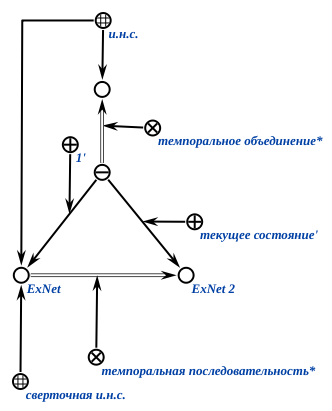
\includegraphics[scale=0.8]{author/part3/figures/temporal_neural_network_scg.png}
	\caption{Темпоральность нейронной сети}
	\label{fig:temporal_neural_network_scg}
\end{figure}

Далее более подробно рассмотрим действие по обучению \scnkeyword{и.н.с.} и сделаем обзор основных методов, применяемых для обучения.

Действие обучения  \scnkeyword{и.н.с.} -- действие, в ходе которого реализуется определенный метод обучения  \scnkeyword{и.н.с.} с заданными параметрами обучения  \scnkeyword{и.н.с.}, методом оптимизации и функцией потерь.

При обучении возможно возникновение следующих проблем:

\begin{itemize}
	\item Переобучение -- проблема, возникающая при обучении  \scnkeyword{и.н.с.}, заключающаяся в том,
	что сеть хорошо адаптируется к паттернам входной активности из обучающей выборки, при этом теряя способность к обобщению.
	Переобучение возникает из-за применения неоправданно сложной модели при обучении  \scnkeyword{и.н.с.} Это происходит,
	когда количество настраиваемых параметров и.н.с. намного больше размера обучающей выборки. Возможные
	варианты решения проблемы заключаются в упрощении модели, увеличении выборки, использовании регуляризации
	(параметр регуляризации, техника dropout и т.д.).\\
	Обнаружение переобученности сложнее, чем недообученности. Как правило, для этого применяется
	кросс-валидация на валидационной выборке, позволяющая оценить момент завершения процесса обучения.
	Идеальным вариантом является достижение баланса между переобученностью и недообученностью.
	
	\item Недообучение -- проблема, возникающая при обучении  \scnkeyword{и.н.с.}, заключающаяся в том,
	что сеть дает одинаково плохие результаты на обучающей и контрольной выборках.
	Чаще всего такого рода проблема возникает при недостаточном времени, затраченном на обучение модели.
	Однако это может быть вызвано и слишком простой архитектурой модели либо малым размером обучающей
	выборки. Соответственно решение, которое может быть принято ML-инженером, заключается в устранении
	этих недостатков: увеличение времени обучения, использование модели с большим числом настраиваемых
	параметров, увеличение размера обучающей выборки, а также уменьшение регуляризации и более тщательный
	отбор признаков для обучающих примеров.
\end{itemize}

Методом обучения \scnkeyword{и.н.с.} называется процесс итеративного поиска оптимальных значений настраиваемых параметров и.н.с., минимизирующих некоторую заданную функцию потерь.

Стоит отметить, что хотя целью применения метода обучения является минимизация функции потерь, ``полезность'' полученной после обучения модели можно оценить только по достигнутому уровню ее обобщающей способности.

Методы обучения могут быть поделены на две большие группы -- \textit{\textbf{методы обучения с учителем}} и \textit{\textbf{методы обучения без учителя}} (контролируемый и неконтролируемый методы обучения).

Метод обучения с учителем -- метод обучения с использованием заданных целевых переменных.

Одним из методов обучения с учителем является метод обратного распространения ошибки.

Приведем его описание в виде алгоритма:

\begin{algorithm}[H]
	\KwData{$X$ -- данные, $E_t$ -- желаемый отклик (метки), $E_m$ -- желаемая ошибка (в соответствии с выбранной функцией потерь)}
	\KwResult{обученная нейронная сеть \textit{Net}}
	инициализация весов \textit{W} и порогов \textit{T};\\
	\Repeat{$E<E_m$}{
		\ForEach{$x \in X$, $e \in E_t$}{
			фаза прямого распространения сигнала: вычисляются активации для всех слоев и.н.с.;\\
			фаза обратного распространения ошибки: вычисляются ошибки для последнего слоя и всех предшествующих слоев;\\
			изменение настраиваемых параметров и.н.с. в соответствии с вычисленными ошибками;\\
		}
		вычисление общей ошибки E на данной эпохе;
	}
\end{algorithm}

Метод обратного распространения ошибки использует заданный метод оптимизации и заданную функцию потерь для реализации фазы обратного распространения ошибки и изменения настраиваемых параметров и.н.с. Одним из самых распространенных методов оптимизации является метод стохастического градиентного спуска. Приведенный метод используется для реализации последовательного варианта обучения.

Следует также отметить, что несмотря на то, что метод отнесен к методам обучения с учителем, в случае
его использования для обучения автокодировщиков в классических публикациях он рассматривается как
метод обучения без учителя, поскольку в данном случае размеченные данные отсутствуют.

\textbf{\textit{Метод обучения без учителя}} -- метод обучения без использования заданных целевых переменных (в режиме самоорганизации)

В ходе выполнения алгоритма метода обучения без учителя выявляются полезные структурные свойства
набора. Неформально его понимают как метод для извлечения информации из распределения, выборка для которого
не была вручную аннотирована человеком [\scncite{Goodfellow2017}]. Метод обучения без учителя может рассматриваться как вспомогательный метод для начальной инициализации настраиваемых параметров и.н.с. В этом случае он является методом предобучения.

Среди методов, применяемых для оптимизации целевой функции можно выделить следующие:

\begin{itemize}
	\item SGD (стохастический градиентный спуск): в данном методе корректировка настраиваемых параметров и.н.с. выполняется в направлении максимального уменьшения функции стоимости, т.е. в направлении, противоположном вектору градиента функции потерь [\scncite{Haykin2006}]
	\item метод Нестерова: Обучение методом стохастического градиентного спуска иногда происходит очень медленно. Импульсный метод позволяет ускорить обучение, особенно в условиях высокой кривизны, небольших, но устойчивых градиентов или зашумленных градиентов. В импульсном методе вычисляется экспоненциально затухающее скользящее среднее прошлых градиентов и продолжается движение в этом направлении. Метод Нестерова является вариантом импульсного алгоритма, в котором градиент вычисляется после применения текущей скорости [\scncite{Goodfellow2017}]
	\item AdaGrad: Данный метод по отдельности адаптирует скорости обучения всех настраиваемых параметров и.н.с., умножая их на коэффициент, обратно пропорциональный квадратному корню из суммы всех прошлых значений квадрата градиента [\scncite{Duchi2011}]
	\item RMSProp: Данный метод является модификацией AdaGrad, которая позволяет улучшить его поведение в невыпуклом случае путем изменения способа агрегирования градиента на экспоненциально взвешенное скользящее среднее. Использование экспоненциально взвешенного скользящего среднего гарантирует повышение скорости сходимости после обнаружения выпуклой впадины, как если бы внутри этой впадины алгоритм AdaGrad был инициализирован заново [\scncite{Goodfellow2017}]
	\item Adam: Данный метод можно рассматривать как комбинацию RMSProp и AdaGrad [\scncite{Kingma2014}]. Помимо усредненного первого момента, данный метод использует усредненное значение вторых моментов градиентов
\end{itemize} 

Отметим, что успешность применения методов оптимизации зависит главным образом от знакомства пользователя с соответствующим алгоритмом [\scncite{Goodfellow2017}].

Еще одним важным компонентом, влияющим на процесс обучения, является используемая функция потерь.

\scnkeyword{Функция потерь} -- функция, используемая для вычисления ошибки, рассчитываемой как разница между фактическим эталонным значением и прогнозируемым значением, получаемым \scnkeyword{и.н.с.}

Среди функций потерь, используемые в качестве целевых функций для применяемого метода оптимизации, можно выделить:

\begin{itemize}
	\item MSE -- средняя квадратичная ошибка\\
		\begin{equation*}
			MSE = \frac{1}{L} \sum_{l=1}^L \sum_{i=1}^m (y_i^l - e_i^l)^2
		\end{equation*}
		где $y_i^l$ -- прогноз модели, $e_i^l$ -- ожидаемый (эталонный) результат, \textit{m} -- размерность выходного вектора, \textit{L} -- объем обучающей выборки.

	\item BCE -- бинарная кросс-энтропия\\
	\begin{equation*}
		BCE = - \sum_{l=1}^L (e^l \log(y^l) + (1 - e^l)\log(1 - y^l))
	\end{equation*}
	где $y^l$ -- прогноз модели, $e^l$ -- ожидаемый (эталонный) результат: \textit{0} или \textit{1}, \textit{L} -- объем обучающей выборки.
	\item MCE -- мультиклассовая кросс-энтропия\\
	\begin{equation*}
		MCE = - \sum_{l=1}^L \sum_{i=1}^m e_{i}^l \log(y_{i}^l)
	\end{equation*}
	где $y_{i}^l$ -- прогноз модели, $e_i^l$ -- ожидаемый (эталонный результат), \textit{m} -- размерность выходного вектора
\end{itemize}

Отметим, что для бинарной кросс-энтропии в выходном слое \scnkeyword{и.н.с.} будет находиться один нейрон, а для для мультиклассовой кросс-энтропии количество нейронов в выходном \scnkeyword{слое и.н.с.} совпадает с количеством классов.

Для решения задачи классификации рекомендуется использовать бинарную или мультиклассовую кросс-энтропийную функцию потерь, для решения задачи регрессии рекомендуется использовать среднюю квадратичную ошибку.

Действие обучения \scnkeyword{и.н.с.} можно проиллюстрировать следующим изображением \textit{\nameref{fig:ann_training_nn_scg}}.

\begin{figure}[H]
	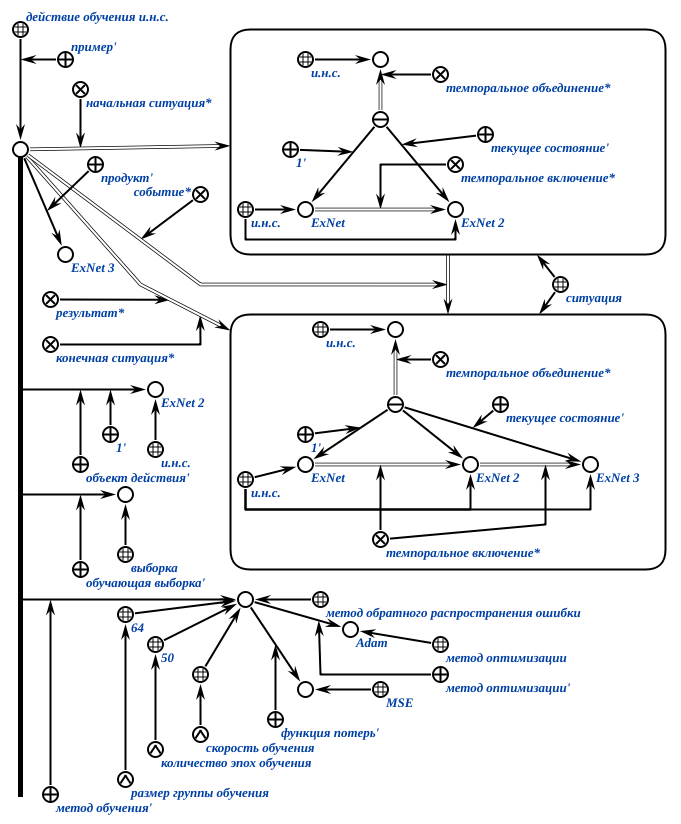
\includegraphics[scale=0.8]{author/part3/figures/ann_training_nn_scg.png}
	\caption{Действие обучения и.н.с.}
	\label{fig:ann_training_nn_scg}
\end{figure}

\section{Логико-семантическая модель ostis-системы автоматизации проектирования искусственных нейронных сетей, семантически совместимых с базами знаний ostis-систем}



\section{Применение глубоких нейронных сетей в интеллектуальных компьютерных системах нового поколения}

Хотя строгого определения понятия глубокая нейронная сеть не существует, ее можно определить как \scnkeyword{и.н.с.} произвольной архитектуры, имеющую более двух скрытых слоев нейронных элементов. В настоящий момент глубокой фактически можно считать любую \scnkeyword{и.н.с.}, на которую не накладывается условие ограничения глубины. Долгое время нейронные сети с более чем двумя скрытыми слоями не изучались и не находили практического применения по причине того, что их обучение классическими подходами (в частности, с помощью метода обратного распространения ошибки) было неэффективно. Это прежде всего связывалось с проблемой ``исчезающего градиента'', которая проявляется в том, что при обучении нейронной сети с большим количеством слоев методом обратного распространения ошибки значения градиентов весовых коэффициентов первых слоев сети быстро становятся близкими к нулю значениями, что приводит к несущественному изменению таких коэффициентов в процессе обучения \cite{n5}. Подобное явление замедляло процесс обучения, делая практическое применение подобных архитектур нецелесообразным. Однако, проводя аналогии с многоуровневыми нейронными архитектурами в человеческом мозге (в частности, со строением вентральной зрительной системы), было понятно, что подобный тип \scnkeyword{и.н.с.} обладает  уникальными и интересными свойствами, позволяя формировать многоуровневую иерархию признаков.

Известный британский информатик Джеффри Хинтон, исследовавший глубокие нейросети доверия [\scncite{}], в 2006 году предложил <<жадный>> алгоритм послойного предобучения глубоких нейронных сетей (greedy layer-wise algorithm) [\scncite{Hinton2006}], основанный на применении \scnkeyword{ограниченных машин Больцмана}, последовательно формируемых и обучаемых из слоев нейросети. Предложенный подход стал поворотным моментом в изучении глубоких нейронных сетей. Последовавший за этим открытием всплеск количества работ, посвященных обучению глубоких сетей, позволил в течение последующих лет улучшить полученные результаты. 

Так, в частности, в 2015 году Я. ЛеКуном было предложено обучать глубокие и.н.с. с использованием альтернативной функции активации ReLU (Rectified Linear Unit - исправленный линейный элемент) [\scncite{LeCun2015}].  Это позволило обучать и.н.с. с нуля на большом количестве исходных данных и при наличии аппаратных возможностей за приемлемое время.

Использование ReLU помогает решить проблему исчезающего градиента, плохого локального минимума и нестабильного градиента путем большей линейности такого типа функций активации [\scncite{}].

Сейчас можно говорить, что существует два альтернативных подхода к обучению глубоких нейросетей: первый предполагает проведение предобучения по хинтоновскому типу, второй -- специальных типов функций активации (ReLU), большой доступной обучающей выборки и некоторых специальных регуляризационных техник (например, dropout).

Выбор того или иного подхода к обучению глубоких нейронных сетей зависит от размера обучающей выборки. Так, если выборка большая, применяется стохастический градиентый спуск с функцией ReLU. В противном случае находит применение подход с предобучением глубокой нейронной сети. Для малых обучающих выборок предобучение позволяет преодолеть переобучение [\scncite{LeCun2015}].

При этом следует отличать предобучение как предварительно выполняемую процедуру в соответствии с хинтоновским подходом (назовем его предобучением I типа) и предобучение как процесс подготовки т.н. предобученной и.н.с., которая может быть дообучена на отличной от исходной выборке для решения других задач (предобучение II типа). Во втором случае может применяться традиционные методики обучения (например, стохастический градиентный спуск с ReLU-функциями активации). Дообучение предобученных моделей может осуществляться на выборке, отличной от исходной выборки, на которой обучалась данная сеть. При этом начальная ошибка, с которой начинается такое дообучение, существенно ниже, чем при использовании ``training from the scratch'' (``обучение с нуля''). Данный подход носит название ``transfer learning'' [\scncite{}]. 

\subsection{Применение предобучения для глубоких нейросетевых моделей}

Существует два основных подхода к предобучению глубоких нейронных сетей I типа. Первый -- метод Хинтона, основанный на применении ограниченных машин Больцмана для предобучения сети. Второй подход базируется на обучении автоэнкодерных нейронных сетей, формируемых также, как и в первом подходе, из структуры исходной сети [\scncite{Bengio2007}]. 

В независимости от используемого подхода, процесс предообучения в общем случае состоит из двух этапов: 
\begin{itemize}
	\item Предобучение нейронной сети методом послойного обучения, начиная с первого слоя  (pre-training). Такое обучение осуществляется без учителя;
	\item Настройка синаптических связей всей сети (fine-tuning) при помощи алгоритма обратного распространения ошибки или алгоритма <<бодрствования и сна>> (wake-sleep algorithm) [\scncite{}].
\end{itemize}

Рассматрим более подробно подход к предобучению с использованием ограниченных машин Больцмана.

Сначала дадим формализованное описание ограниченной машины Больцмана.

\begin{SCn}
	\scnheader{ограниченная машина Больцмана}
	\scnidtf{restricted Boltzmann Machine}
	\scnidtf{RBM}
	\scnidtf{ограниченная машина Больцмана}
	\scnsubset{искусственная нейронная сеть}
	\scntext{пояснение}{\scnkeyword{и.н.с.}, состоящая из двух слоев стохастических бинарных нейронных элементов, которые соединены между собой двунаправленными симметричными связями}
\end{SCn}

Входной слой нейронных элементов RBM называется видимым (слой $X$), а выходной -- скрытым (слой $Y$). Ограниченная машина Больцмана может генерировать любое дискретное распределение, если используется достаточное количество нейронов скрытого слоя [\scncite{n5}].

Схема RBM представлена на рисунке \textit{\nameref{fig:rbm_scheme}}.

\begin{figure}[H]
	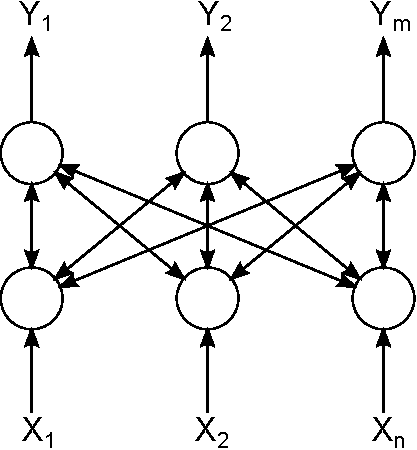
\includegraphics[width=0.4\textwidth]{author/part3/figures/pic1-3.pdf}
	\caption{Ограниченная машина Больцмана}
	\label{fig:rbm_scheme}
\end{figure}

Данная сеть является стохастической нейронной сетью, в которой состояния видимых и скрытых нейронов меняются в соответствии с вероятностной версией сигмоидной функции активации:

\begin{equation}
	p(y_j\lvert x)=\frac{1}{1+e^{-S_j}},\ S_j=\sum_i^n w_{ij}x_i+T_j
\end{equation}

\begin{equation}
	p(x_i\lvert y)=\frac{1}{1+e^{-S_i}},\ S_i=\sum_j^m w_{ij}y_j+T_i
\end{equation}

Состояния видимых и скрытых нейронных элементов принимаются независимыми:

\begin{equation*}
	\begin{aligned}
		P(x \lvert y) = \prod_{i=1}^n P(x_i \lvert y)\\
		P(y \lvert x) = \prod_{j=1}^m P(y_j \lvert x)
	\end{aligned}	
\end{equation*}

Таким образом, состояния всех нейронных элементов ограниченной машины Больцмана определяются через распределение вероятностей. В RBM нейроны скрытого слоя являются детекторами признаков, которые сохраняют закономерности входных данных. Основная задача обучения состоит в воспроизведении распределения входных данных на основе состояний нейронов скрытого слоя как можно точнее. Это эквивалентно  максимизации функции правдоподобия путем модификации синаптических связей нейронной сети. Рассмотрим этот процесс подробнее. 
Вероятность нахождения видимого и скрытого нейрона в состоянии $(x, y)$ определяется на основе распределения Гиббса:

\begin{equation*}
	P(x, y)=\frac{e^{-E(x,y)}}{Z}
\end{equation*}
где $E(x,y)$ -- энергия системы в состоянии $(x,y)$, $Z$ -- параметр, который определяет условие нормализации вероятностей, то есть, чтобы сумма вероятностей равнялась единице. Данный параметр определяется следующим образом:

\begin{equation*}
	Z=\sum_{x,y} e^{-E(x,y)}
\end{equation*}

Вероятность нахождения видимых нейронов в определенном состоянии равняется сумме вероятностей  конфигураций $P(x,y)$ по состояниям скрытых нейронов:

\begin{equation*}
	P(x)=\sum_y P(x,y)=\sum_y \frac{e^{-E(x,y)}}{Z}=\frac{\sum_y e^{-E(x,y)}}{\sum_{x,y} e^{-E(x,y)}}
\end{equation*}

Для нахождения правила модификации синаптических связей необходимо максимизировать вероятность воспроизведения состояний видимых нейронов $P(x)$ ограниченной машиной Больцмана. Для того, чтобы определить максимум функции правдоподобия распределения данных $P(x)$ будем использовать метод градиентного спуска в пространстве весовых коэффициентов и пороговых значений сети, где в качестве целевой функции будем использовать функцию логарифмического правдоподобия:

\begin{equation*}
	\ln P(x)=\ln \sum_y e^{-E(x,y)}-\ln \sum_{x,y} e^{-E(x,y)}
\end{equation*}

Тогда градиент равен

\begin{equation*}
	\frac{\partial \ln P(x)}{\partial w_{ij}}=\frac{\partial}{\partial w_{ij}}\ln \sum_y e^{-E(x,y)}-\frac{\partial}{\partial w_{ij}}\ln\sum_{x,y} e^{-E(x,y)}
\end{equation*}

Преобразуя последнее выражение, получим

\begin{equation*}
	\frac{\partial \ln P(x)}{\partial w_{ij}}=-\frac{1}{\sum_y e^{-E(x,y)}}\sum_y e^{-E(x,y)}\frac{\partial E(x,y)}{\partial w_{ij}}+\frac{1}{\sum_{x,y} e^{-E(x,y)}}\sum_{x,y} e^{-E(x,y)}\frac{\partial E(x,y)}{\partial w_{ij}}
\end{equation*}

Так как

\begin{equation*}
	P(x,y)=P(y \lvert x)P(x)
\end{equation*}

то

\begin{equation*}
	P(y \lvert x) = \frac{P(x,y)}{P(x)}=\frac{\frac{1}{Z}e^{-E(x,y)}}{\frac{1}{Z}\sum_y e^{-E(x,y)}}=\frac{e^{-E(x,y)}}{\sum_y e^{-E(x,y)}}
\end{equation*}

В результате можно получить следующее выражение:

\begin{equation}
	\label{derivative_log}
	\frac{\partial \ln P(x)}{\partial w_{ij}}=-\sum_y P(y \lvert x)\frac{\partial E(x,y)}{\partial w_{ij}} + \sum_{x,y} P(x,y)\frac{\partial E(x,y)}{\partial w_{ij}}
\end{equation}

В данном выражении первое слагаемое определяет позитивную фазу работы машины Больцмана, когда сеть работает на основе образов из обучающей выборки. Второе слагаемое характеризует негативную фазу функционирования, когда сеть работает в свободном режиме независимо от окружающей среды.

Рассмотрим энергию сети RBM. С такой точки зрения задача обучения состоит в том, чтобы на основе входных данных найти конфигурацию выходных переменных с минимальной энергией. В результате на обучающем множестве сеть будет иметь меньшую энергию по сравнению с другими состояниями. Функция энергии бинарного состояния $(x,y)$ определяется аналогично энергетической функции сети Хопфилда:

\begin{equation}
	E(x,y)=-\sum_i x_iT_i-\sum_j y_jT_j-\sum_{i,j} x_iy_jw_{ij}
\end{equation}

В этом случае

\begin{equation*}
	\frac{\partial E(x,y)}{\partial w_{ij}}=-x_iy_j 	
\end{equation*}

Подставляя полученное значение в формулу \ref{derivative_log}, получим

\begin{equation}
	\label{grad_weights}
	\frac{\partial \ln P(x)}{\partial w_{ij}}=\sum_y P(y \lvert x)x_i y_j-\sum_{x,y} P(x,y)x_iy_j
\end{equation}

Так как математическое ожидание равняется:

\begin{equation}
	\label{mean}
	E(x)=\sum_i x_iP_i
\end{equation}	  

то

\begin{equation*}
	\frac{\partial \ln P(x)}{\partial w_{ij}}=E\left[x_iy_j\right]_{data}-E\left[x_iy_j\right]_{model}
\end{equation*}

Рассуждая аналогичным образом, находим

\begin{equation*}
	\frac{\partial \ln P(x)}{\partial T_{i}}=-\sum_y P(y \lvert x)\frac{\partial E(x,y)}{\partial T_{i}} + \sum_{x,y} P(x,y)\frac{\partial E(x,y)}{\partial T_{i}}
\end{equation*}

и

\begin{equation*}
	\frac{\partial \ln P(x)}{\partial T_{j}}=-\sum_y P(y \lvert x)\frac{\partial E(x,y)}{\partial T_{j}} + \sum_{x,y} P(x,y)\frac{\partial E(x,y)}{\partial T_{j}}
\end{equation*}

Так как

\begin{equation*}
	\frac{\partial E(x,y)}{\partial T_{i}}=-x_i 
\end{equation*}

и 

\begin{equation*}
	\frac{\partial E(x,y)}{\partial T_{j}}=-y_j 
\end{equation*}

то, учитывая формулу \ref{mean}, получим градиенты для пороговых значений:

\begin{equation}
	\label{grad_biases}
	\begin{aligned}
		\frac{\partial \ln P(x)}{\partial T_i}=E\left[x_i\right]_{data}-E\left[x_i\right]_{model}\\
		\frac{\partial \ln P(x)}{\partial T_j}=E\left[y_j\right]_{data}-E\left[y_j\right]_{model}
	\end{aligned}
\end{equation}

Как следует из последних выражений, первое слагаемое характеризует работу сети на основе данных из обучающей выборки, а  второе слагаемое характеризует работу сети на основе данных модели (данные генерируемые сетью), то есть в свободном режиме независимо от окружающей среды.
Так как вычисление математического ожидания в формулах \ref{grad_weights} и \ref{grad_biases} является сложной задачей, Хинтон предложил использовать аппроксимацию данных слагаемых, получаемую применением процедуры, которую он назвал контрастным расхождением (Contrastive Divergence (CD)) [\scncite{n1}].

Такая аппроксимация основывается на дискретизаторе Гиббса (Gibbs sampling). В этом случае первые слагаемые в выражениях \ref{grad_weights} и \ref{grad_biases} характеризуют распределение данных в момент времени $t=0$, а вторые слагаемые характеризуют реконструированные или генерируемые моделью состояния в момент времени $t=k$. Исходя из этого, CD-$k$ процедура может быть представлена следующим образом:

\begin{equation}
	x(0) \rightarrow y(0) \rightarrow x(1) \rightarrow y(1) \rightarrow \ldots \rightarrow x(k) \rightarrow y(k)
\end{equation}

В результате можно сформулировать следующие правила для обучения RBM сети. В случае применения CD-1 (случай $k=1$) и, учитывая, что в соответствии с методом градиентного подъема

\begin{equation*}
	w_{ij}(t+1)=w_{ij}(t)+\alpha\frac{\partial \ln P(x)}{\partial w_{ij}(t)}
\end{equation*}	 

Можно получить, что
\begin{equation*}
	w_{ij}(t+1)=w_{ij}(t)+\alpha(x_i(0)y_j(0)-x_i(1)y_j(1))
\end{equation*}
\begin{equation*}		
	T_i(t+1)=T_i(t)+\alpha(x_i(0)-x_i(1))
\end{equation*}
\begin{equation*}		
	T_j(t+1)=T_j(t)+\alpha(y_j(0)-y_j(1)).
\end{equation*}		

Аналогичным образом, для алгоритма  CD-$k$
\begin{equation*}
	w_{ij}(t+1)=w_{ij}(t)+\alpha(x_i(0)y_j(0)-x_i(k)y_j(k))
\end{equation*} 
\begin{equation*}	
	T_i(t+1)=T_i(t)+\alpha(x_i(0)-x_i(k))
\end{equation*} 
\begin{equation*}		
	T_j(t+1)=T_j(t)+\alpha(y_j(0)-y_j(k)).
\end{equation*} 

Из последних выражений видно, что в процессе обучения ограниченной машины Больцмана минимизируется разница между оригинальными данными и данными, генерируемыми моделью.

Суммируя вышесказанное, приведем полный алгоритм обучения RBM для случая CD-1 (алгоритм~\ref{rbm_learning}).

\begin{algorithm}
	\SetAlgoLined
	
	\KwData{$x_i(0)$ -- образ из обучающей выборки\newline
		$\alpha$ - скорость обучения
	}
	\KwResult{матрица весовых коэффициентов $W$, вектор порогов видимых элементов $b$, вектор порогов скрытых нейронов $c$}
	\ForEach{скрытого нейрона $j$}{
		Вычислить $P(y_{j}(0)=1|x_{i}(0))$ (для биномиальных нейронов sigm($\sum_{i}{w_{ij}x_{i}(0)}+T_j$))\;
		Генерировать $y_{j}(0) \in \{0, 1\}$ из $P(y_{j}(0)|x_i(0))$\;
	}
	\ForEach{видимого нейрона $i$}
	{
		Вычислить $P(x_{i}(1)=1|y_j(0))$ (для биномиальных нейронов sigm($\sum_{j}{w_{ij}y_{j}(0)} + T_i$))\;
		Генерировать $x_{i}(1) \in \{0, 1\}$ из $P(x_{i}(1)|y_j(0)$\;
	}	
	\ForEach{скрытых нейронов $j$}
	{
		Вычислить $P(y_{j}(1)=1|x_i(1))$ (для биномиальных нейронов sigm($\sum_{i}{w_{ij}x_{i}(1)} + T_j$))\;
	}
	$W \leftarrow W + \alpha(x(0)y(0)' - x(1)P(y(1)=1|x(1))')$\;
	$T_i \leftarrow T_i + \alpha(x(0) - x(1))$\;
	$T_j \leftarrow T_j + \alpha(y(0) - P(y(1)=1|x(1)))$\;
	\caption{Процедура обучения RBM}
	\label{rbm_learning}
\end{algorithm}

\subsection{Алгоритм обучения ГНС} \label{subsect1_3_2}

Обучение нейронной сети глубокого доверия происходит на основе <<жадного>> алгоритма послойного обучения (greedy layer-wise algorithm). В соответствии с ним вначале обучается первый слой сети как RBM. Для этого входные данные поступают на видимый слой нейронных элементов и используя CD-$k$ процедуру вычисляются состояния скрытых $p(y \lvert x)$ и видимых нейронов $p(x \lvert y)$. В процессе выполнения данной процедуры (не более 100 эпох) изменяются весовые коэффициенты и пороговые значения RBM сети, которые затем фиксируются (алгоритм \ref{rbm_learning}). Затем берется второй слой нейронной сети и конструируется новая RBM. Входными данными для нее являются данные с предыдущего слоя. Происходит обучение и процесс продолжается для всех последующих слоев нейронной сети, как показано на рисунке~\ref{fig:pic1_4}. В результате такого обучения без учителя можно получить приемлемую начальную инициализацию настраиваемых параметров сети глубокого доверия. На заключительном этапе осуществляется <<тонкая>> настройка параметров всей сети при помощи алгоритма обратного распространения ошибки или алгоритма <<бодрствования и сна>> (wake-sleep algorithm). 

\begin{figure}[H]
	\centering
	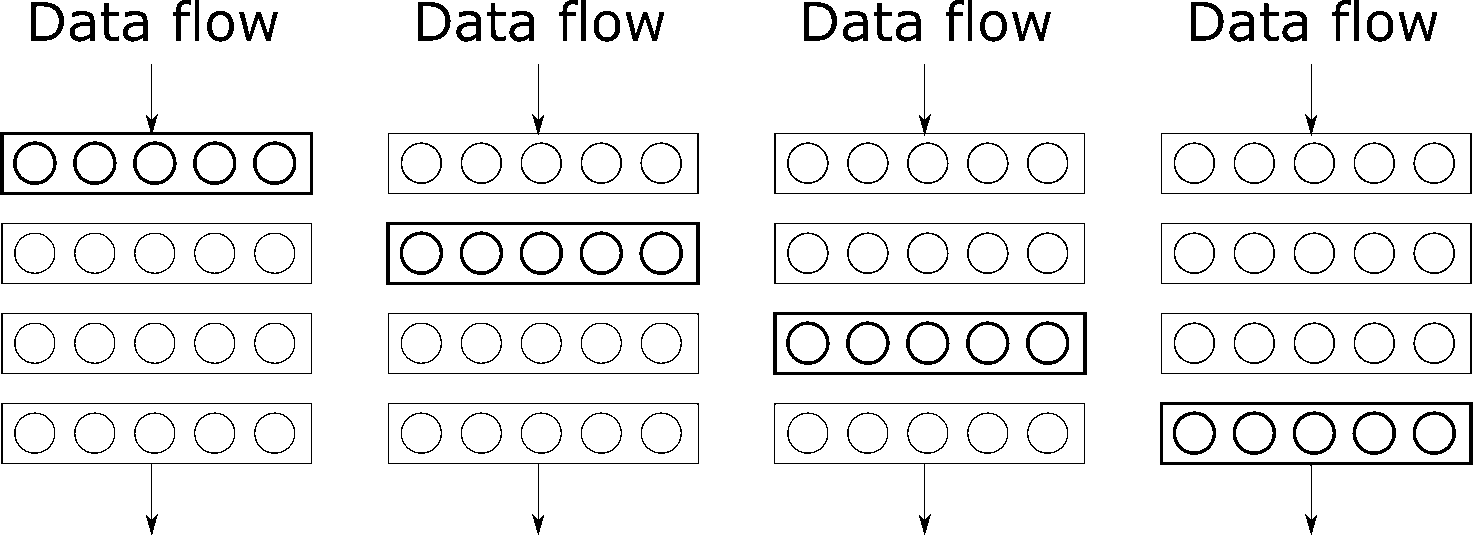
\includegraphics[width=\textwidth]{author/part3/figures/pic1-4.png}
	\caption{<<Жадный>> алгоритм послойного обучения}
	\label{fig:pic1_4}
\end{figure}

\section{Этап <<тонкой>> настройки глубокой НС}

На этапе тонкой настройки нейронной сети, называемой fine-tuning, выполняется обучение всей сети некоторым традиционным подходом (например, алгоритмом обратного распространения ошибки или <<бодрствования и сна>>).

Критически важным для этого этапа является начальная инициализация весов и порогов. Если такая инициализация выполнена в ходе предобучения, то сеть начинает процесс тонкой настройки с <<хороших>> начальных значений, что обуславливает быструю сходимость.

Если же предобучение отсутствует и используется традиционная <<поверхностная>> схема обучения со случайной инициализацией параметров, обучение сети может быстро остановиться и, как результат, приемлемая обобщающая способность не будет достигнута.

Не менее важным является правильный выбор критерия обучения. Наиболее известными и используемыми в настоящий момент функциями ошибок являются функция среднеквадратичной ошибки (MSE):

\begin{equation}
	\label{MSE}
	E_{MSE} = \frac{1}{2}\sum_{j=1}^{n}(y_j - t_j)^2
\end{equation}
и кросс-энтропийная функция (CE):

\begin{equation}
	\label{CE_multiclass}
	E_{CE_{mult}} = -\sum_{j=1}^{n}t_j\log(y_j)
\end{equation}
где $n$ -- количество нейронных элементов в последнем слое, $y_j$ -- выход нейрона $j$, $t_j$ -- эталонное значение этого нейрона, множитель $\frac{1}{2}$ введен для удобства вычислений.

Формула \ref{MSE} справедлива для одного обучающего примера. Для $L$ обучающих примеров она запишется в следующем виде:

\begin{equation}
	\label{MSE_L}
	E_{MSE} = \frac{1}{2L}\sum_{i=1}^{L}\sum_{j=1}^{n}(y_j^i - t_j^i)^2	
\end{equation}

Далее всюду, если не оговорено особо, мы будем использовать формулу \ref{MSE}.

На практике вместо формулы \ref{CE_multiclass} для мультиклассового случая часто применяется формула, обобщающая двухклассовый случай:

\begin{equation}
	\label{CE}
	E_{CE} = -\sum_{j=1}^n(t_j\log(y_j) + (1-t_j)\log(1-y_j))
\end{equation}

В соответствии с методом обратного распространения, для настройки весовых коэффициентов и порогов применяются следующие правила:

\begin{equation}
	w_{i-1,i} = w_{i-1, i} - \alpha \frac{\partial E}{\partial w_{i-1, i}}
\end{equation}
\begin{equation}
	T_i = T_i - \alpha \frac{\partial E}{\partial T_i}
\end{equation}
где $i=1..N$, $N$ -- количество обрабатывающих слоев нейронной сети, $\alpha$ -- скорость обучения, а соответствующие градиенты находятся по формулам:

\begin{equation}
	\label{weights_delta}
	\frac{\partial E}{\partial w_{i-1, i}} = \frac{\partial E}{\partial S_i} y_{i-1}
\end{equation}
\begin{equation}
	\label{biases_delta}
	\frac{\partial E}{\partial T_i} = \frac{\partial E}{\partial S_i}
\end{equation}

Частные производные по взвешенным суммам $S_i$ получаются в соответствии со следующими выражениями:
\begin{equation}
	\label{last_layer_error}
	\frac{\partial E}{\partial S_l} = (y_l - t_l)F'(S_l)
\end{equation}

\begin{equation}
	\label{sum_rec_common}
	\frac{\partial E}{\partial S_{i-1}} = \Bigg(\sum_{i}\frac{\partial E}{\partial S_i}w_{i-1, i}\Bigg)F'(S_{i-1})
\end{equation}
где $F$ -- функция активации нейронных элементов, $l$ -- индекс последнего слоя нейронной сети.

Формула \ref{last_layer_error} актуальна для случая, если используется целевая функция $E_{MSE}$. Для случая $E_{CE}$ она будет иметь такой вид:

\begin{equation}
	\label{last_layer_error_ce}
	\frac{\partial E}{\partial S_l} = \frac{y_l - t_l}{y_l(1-y_l)}F'(S_l)
\end{equation}

В случае использования логистической функции, формула \ref{last_layer_error_ce} упрощается:

\begin{equation}
	\frac{\partial E}{\partial S_l} = y_l - t_l
\end{equation}

Формулы \ref{weights_delta}, \ref{biases_delta} и \ref{sum_rec_common} справедливы как для случая $E_{CE}$, так и для $E_{MSE}$.

Для $E_{CE_{mult}}$ эти формулы справедливы для функции активации \textbf{softmax} на последнем слое нейронной сети. Покажем это.

Имеем

\begin{equation}
	\label{common_E}
	\frac{\partial E_{CE_{mult}}}{\partial S_l} = \sum_{k=1}^{n} \frac{\partial E_{CE_{mult}}}{\partial y_k}\frac{\partial y_k}{\partial S_l} = \frac{\partial E_{CE_{mult}}}{\partial y_l}\frac{\partial y_l}{\partial S_l} + \sum_{k\neq l}\frac{\partial E_{CE_{mult}}}{\partial y_k}\frac{\partial y_k}{\partial S_l}
\end{equation}

Очевидно, 
\begin{equation}
	\label{part_deriv_y}
	\frac{\partial E_{CE_{mult}}}{\partial y_l} = -\frac{t_l}{y_l}
\end{equation}

Учитывая
\begin{equation}
	y_l = \frac{e^S_l}{\sum_{k=1}^{n} e^S_k}
\end{equation}
где $l$ -- индекс последнего слоя сети, $S_l$ -- соответствующая взвешенная сумма, найдем значения частной производной $\frac{\partial y_l}{\partial S_k}$.
\begin{itemize}
	\item Случай $l = k$
	\begin{multline}
		\label{part1_deriv_S}
		\frac{\partial y_l}{\partial S_l} = \frac{e^{S_l}\sum e^{S_k} - e^{2S_l}}{(\sum e^{S_k})^2} = \\ = \frac{e^{S_l}\sum e^{S_k}}{(\sum e^{S_k})^2}-\frac{e^{2S_l}}{(\sum e^{S_k})^2}=y_l - y_l^2 = y_l(1-y_l)
	\end{multline}
	\item $l \neq k$
	\begin{equation}
		\label{part2_deriv_S}
		\frac{\partial y_l}{\partial S_k} = -e^{S_l}\Big(\sum e^{S_k}\Big)^{-2}e^{S_k} = -y_ly_k
	\end{equation}
\end{itemize}

Подставляя полученные выражения \ref{part1_deriv_S}, \ref{part2_deriv_S} и \ref{part_deriv_y} в \ref{common_E}, получим
\begin{equation}
	\frac{\partial E_{CE_{mult}}}{\partial S_l} = -t_l(1-y_l) + \sum_{k\neq l}t_ky_l = -t_l + y_l\sum_{k=1}^{n}t_k = y_l - t_l
\end{equation}

%%%%%%%%%%%%%%%%%%%%%%%%% referenc.tex %%%%%%%%%%%%%%%%%%%%%%%%%%%%%%
% sample references
% %
% Use this file as a template for your own input.
%
%%%%%%%%%%%%%%%%%%%%%%%% Springer-Verlag %%%%%%%%%%%%%%%%%%%%%%%%%%
%
% BibTeX users please use
% \bibliographystyle{}
% \bibliography{}
%
\biblstarthook{In view of the parallel print and (chapter-wise) online publication of your book at \url{www.springerlink.com} it has been decided that -- as a genreral rule --  references should be sorted chapter-wise and placed at the end of the individual chapters. However, upon agreement with your contact at Springer you may list your references in a single seperate chapter at the end of your book. Deactivate the class option \texttt{sectrefs} and the \texttt{thebibliography} environment will be put out as a chapter of its own.\\\indent
References may be \textit{cited} in the text either by number (preferred) or by author/year.\footnote{Make sure that all references from the list are cited in the text. Those not cited should be moved to a separate \textit{Further Reading} section or chapter.} If the citatiion in the text is numbered, the reference list should be arranged in ascending order. If the citation in the text is author/year, the reference list should be \textit{sorted} alphabetically and if there are several works by the same author, the following order should be used:
\begin{enumerate}
\item all works by the author alone, ordered chronologically by year of publication
\item all works by the author with a coauthor, ordered alphabetically by coauthor
\item all works by the author with several coauthors, ordered chronologically by year of publication.
\end{enumerate}
The \textit{styling} of references\footnote{Always use the standard abbreviation of a journal's name according to the ISSN \textit{List of Title Word Abbreviations}, see \url{http://www.issn.org/en/node/344}} depends on the subject of your book:
\begin{itemize}
\item The \textit{two} recommended styles for references in books on \textit{mathematical, physical, statistical and computer sciences} are depicted in ~\cite{science-contrib, science-online, science-mono, science-journal, science-DOI} and ~\cite{phys-online, phys-mono, phys-journal, phys-DOI, phys-contrib}.
\item Examples of the most commonly used reference style in books on \textit{Psychology, Social Sciences} are~\cite{psysoc-mono, psysoc-online,psysoc-journal, psysoc-contrib, psysoc-DOI}.
\item Examples for references in books on \textit{Humanities, Linguistics, Philosophy} are~\cite{humlinphil-journal, humlinphil-contrib, humlinphil-mono, humlinphil-online, humlinphil-DOI}.
\item Examples of the basic Springer style used in publications on a wide range of subjects such as \textit{Computer Science, Economics, Engineering, Geosciences, Life Sciences, Medicine, Biomedicine} are ~\cite{basic-contrib, basic-online, basic-journal, basic-DOI, basic-mono}. 
\end{itemize}
}

\begin{thebibliography}{99.}%
% and use \bibitem to create references.
%
% Use the following syntax and markup for your references if 
% the subject of your book is from the field 
% "Mathematics, Physics, Statistics, Computer Science"
%
% Contribution 
\bibitem{science-contrib} Broy, M.: Software engineering --- from auxiliary to key technologies. In: Broy, M., Dener, E. (eds.) Software Pioneers, pp. 10-13. Springer, Heidelberg (2002)
%
% Online Document
\bibitem{science-online} Dod, J.: Effective substances. In: The Dictionary of Substances and Their Effects. Royal Society of Chemistry (1999) Available via DIALOG. \\
\url{http://www.rsc.org/dose/title of subordinate document. Cited 15 Jan 1999}
%
% Monograph
\bibitem{science-mono} Geddes, K.O., Czapor, S.R., Labahn, G.: Algorithms for Computer Algebra. Kluwer, Boston (1992) 
%
% Journal article
\bibitem{science-journal} Hamburger, C.: Quasimonotonicity, regularity and duality for nonlinear systems of partial differential equations. Ann. Mat. Pura. Appl. \textbf{169}, 321--354 (1995)
%
% Journal article by DOI
\bibitem{science-DOI} Slifka, M.K., Whitton, J.L.: Clinical implications of dysregulated cytokine production. J. Mol. Med. (2000) doi: 10.1007/s001090000086 
%
\bigskip

% Use the following (APS) syntax and markup for your references if 
% the subject of your book is from the field 
% "Mathematics, Physics, Statistics, Computer Science"
%
% Online Document
\bibitem{phys-online} J. Dod, in \textit{The Dictionary of Substances and Their Effects}, Royal Society of Chemistry. (Available via DIALOG, 1999), 
\url{http://www.rsc.org/dose/title of subordinate document. Cited 15 Jan 1999}
%
% Monograph
\bibitem{phys-mono} H. Ibach, H. L\"uth, \textit{Solid-State Physics}, 2nd edn. (Springer, New York, 1996), pp. 45-56 
%
% Journal article
\bibitem{phys-journal} S. Preuss, A. Demchuk Jr., M. Stuke, Appl. Phys. A \textbf{61}
%
% Journal article by DOI
\bibitem{phys-DOI} M.K. Slifka, J.L. Whitton, J. Mol. Med., doi: 10.1007/s001090000086
%
% Contribution 
\bibitem{phys-contrib} S.E. Smith, in \textit{Neuromuscular Junction}, ed. by E. Zaimis. Handbook of Experimental Pharmacology, vol 42 (Springer, Heidelberg, 1976), p. 593
%
\bigskip
%
% Use the following syntax and markup for your references if 
% the subject of your book is from the field 
% "Psychology, Social Sciences"
%
%
% Monograph
\bibitem{psysoc-mono} Calfee, R.~C., \& Valencia, R.~R. (1991). \textit{APA guide to preparing manuscripts for journal publication.} Washington, DC: American Psychological Association.
%
% Online Document
\bibitem{psysoc-online} Dod, J. (1999). Effective substances. In: The dictionary of substances and their effects. Royal Society of Chemistry. Available via DIALOG. \\
\url{http://www.rsc.org/dose/Effective substances.} Cited 15 Jan 1999.
%
% Journal article
\bibitem{psysoc-journal} Harris, M., Karper, E., Stacks, G., Hoffman, D., DeNiro, R., Cruz, P., et al. (2001). Writing labs and the Hollywood connection. \textit{J Film} Writing, 44(3), 213--245.
%
% Contribution 
\bibitem{psysoc-contrib} O'Neil, J.~M., \& Egan, J. (1992). Men's and women's gender role journeys: Metaphor for healing, transition, and transformation. In B.~R. Wainrig (Ed.), \textit{Gender issues across the life cycle} (pp. 107--123). New York: Springer.
%
% Journal article by DOI
\bibitem{psysoc-DOI}Kreger, M., Brindis, C.D., Manuel, D.M., Sassoubre, L. (2007). Lessons learned in systems change initiatives: benchmarks and indicators. \textit{American Journal of Community Psychology}, doi: 10.1007/s10464-007-9108-14.
%
%
% Use the following syntax and markup for your references if 
% the subject of your book is from the field 
% "Humanities, Linguistics, Philosophy"
%
\bigskip
%
% Journal article
\bibitem{humlinphil-journal} Alber John, Daniel C. O'Connell, and Sabine Kowal. 2002. Personal perspective in TV interviews. \textit{Pragmatics} 12:257--271
%
% Contribution 
\bibitem{humlinphil-contrib} Cameron, Deborah. 1997. Theoretical debates in feminist linguistics: Questions of sex and gender. In \textit{Gender and discourse}, ed. Ruth Wodak, 99--119. London: Sage Publications.
%
% Monograph
\bibitem{humlinphil-mono} Cameron, Deborah. 1985. \textit{Feminism and linguistic theory.} New York: St. Martin's Press.
%
% Online Document
\bibitem{humlinphil-online} Dod, Jake. 1999. Effective substances. In: The dictionary of substances and their effects. Royal Society of Chemistry. Available via DIALOG. \\
http://www.rsc.org/dose/title of subordinate document. Cited 15 Jan 1999
%
% Journal article by DOI
\bibitem{humlinphil-DOI} Suleiman, Camelia, Daniel C. O'Connell, and Sabine Kowal. 2002. `If you and I, if we, in this later day, lose that sacred fire...': Perspective in political interviews. \textit{Journal of Psycholinguistic Research}. doi: 10.1023/A:1015592129296.
%
%
%
\bigskip
%
%
% Use the following syntax and markup for your references if 
% the subject of your book is from the field 
% "Computer Science, Economics, Engineering, Geosciences, Life Sciences"
%
%
% Contribution 
\bibitem{basic-contrib} Brown B, Aaron M (2001) The politics of nature. In: Smith J (ed) The rise of modern genomics, 3rd edn. Wiley, New York 
%
% Online Document
\bibitem{basic-online} Dod J (1999) Effective Substances. In: The dictionary of substances and their effects. Royal Society of Chemistry. Available via DIALOG. \\
\url{http://www.rsc.org/dose/title of subordinate document. Cited 15 Jan 1999}
%
% Journal article by DOI
\bibitem{basic-DOI} Slifka MK, Whitton JL (2000) Clinical implications of dysregulated cytokine production. J Mol Med, doi: 10.1007/s001090000086
%
% Journal article
\bibitem{basic-journal} Smith J, Jones M Jr, Houghton L et al (1999) Future of health insurance. N Engl J Med 965:325--329
%
% Monograph
\bibitem{basic-mono} South J, Blass B (2001) The future of modern genomics. Blackwell, London 
%
\end{thebibliography}
